\documentclass[1p]{elsarticle_modified}
%\bibliographystyle{elsarticle-num}

%\usepackage[colorlinks]{hyperref}
%\usepackage{abbrmath_seonhwa} %\Abb, \Ascr, \Acal ,\Abf, \Afrak
\usepackage{amsfonts}
\usepackage{amssymb}
\usepackage{amsmath}
\usepackage{amsthm}
\usepackage{scalefnt}
\usepackage{amsbsy}
\usepackage{kotex}
\usepackage{caption}
\usepackage{subfig}
\usepackage{color}
\usepackage{graphicx}
\usepackage{xcolor} %% white, black, red, green, blue, cyan, magenta, yellow
\usepackage{float}
\usepackage{setspace}
\usepackage{hyperref}

\usepackage{tikz}
\usetikzlibrary{arrows}

\usepackage{multirow}
\usepackage{array} % fixed length table
\usepackage{hhline}

%%%%%%%%%%%%%%%%%%%%%
\makeatletter
\renewcommand*\env@matrix[1][\arraystretch]{%
	\edef\arraystretch{#1}%
	\hskip -\arraycolsep
	\let\@ifnextchar\new@ifnextchar
	\array{*\c@MaxMatrixCols c}}
\makeatother %https://tex.stackexchange.com/questions/14071/how-can-i-increase-the-line-spacing-in-a-matrix
%%%%%%%%%%%%%%%

\usepackage[normalem]{ulem}

\newcommand{\msout}[1]{\ifmmode\text{\sout{\ensuremath{#1}}}\else\sout{#1}\fi}
%SOURCE: \msout is \stkout macro in https://tex.stackexchange.com/questions/20609/strikeout-in-math-mode

\newcommand{\cancel}[1]{
	\ifmmode
	{\color{red}\msout{#1}}
	\else
	{\color{red}\sout{#1}}
	\fi
}

\newcommand{\add}[1]{
	{\color{blue}\uwave{#1}}
}

\newcommand{\replace}[2]{
	\ifmmode
	{\color{red}\msout{#1}}{\color{blue}\uwave{#2}}
	\else
	{\color{red}\sout{#1}}{\color{blue}\uwave{#2}}
	\fi
}

\newcommand{\Sol}{\mathcal{S}} %segment
\newcommand{\D}{D} %diagram
\newcommand{\A}{\mathcal{A}} %arc


%%%%%%%%%%%%%%%%%%%%%%%%%%%%%5 test

\def\sl{\operatorname{\textup{SL}}(2,\Cbb)}
\def\psl{\operatorname{\textup{PSL}}(2,\Cbb)}
\def\quan{\mkern 1mu \triangleright \mkern 1mu}

\theoremstyle{definition}
\newtheorem{thm}{Theorem}[section]
\newtheorem{prop}[thm]{Proposition}
\newtheorem{lem}[thm]{Lemma}
\newtheorem{ques}[thm]{Question}
\newtheorem{cor}[thm]{Corollary}
\newtheorem{defn}[thm]{Definition}
\newtheorem{exam}[thm]{Example}
\newtheorem{rmk}[thm]{Remark}
\newtheorem{alg}[thm]{Algorithm}

\newcommand{\I}{\sqrt{-1}}
\begin{document}

%\begin{frontmatter}
%
%\title{Boundary parabolic representations of knots up to 8 crossings}
%
%%% Group authors per affiliation:
%\author{Yunhi Cho} 
%\address{Department of Mathematics, University of Seoul, Seoul, Korea}
%\ead{yhcho@uos.ac.kr}
%
%
%\author{Seonhwa Kim} %\fnref{s_kim}}
%\address{Center for Geometry and Physics, Institute for Basic Science, Pohang, 37673, Korea}
%\ead{ryeona17@ibs.re.kr}
%
%\author{Hyuk Kim}
%\address{Department of Mathematical Sciences, Seoul National University, Seoul 08826, Korea}
%\ead{hyukkim@snu.ac.kr}
%
%\author{Seokbeom Yoon}
%\address{Department of Mathematical Sciences, Seoul National University, Seoul, 08826,  Korea}
%\ead{sbyoon15@snu.ac.kr}
%
%\begin{abstract}
%We find all boundary parabolic representation of knots up to 8 crossings.
%
%\end{abstract}
%\begin{keyword}
%    \MSC[2010] 57M25 
%\end{keyword}
%
%\end{frontmatter}

%\linenumbers
%\tableofcontents
%
\newcommand\colored[1]{\textcolor{white}{\rule[-0.35ex]{0.8em}{1.4ex}}\kern-0.8em\color{red} #1}%
%\newcommand\colored[1]{\textcolor{white}{ #1}\kern-2.17ex	\textcolor{white}{ #1}\kern-1.81ex	\textcolor{white}{ #1}\kern-2.15ex\color{red}#1	}

{\Large $\underline{12a_{0490}~(K12a_{0490})}$}

\setlength{\tabcolsep}{10pt}
\renewcommand{\arraystretch}{1.6}
\vspace{1cm}\begin{tabular}{m{100pt}>{\centering\arraybackslash}m{274pt}}
\multirow{5}{120pt}{
	\centering
	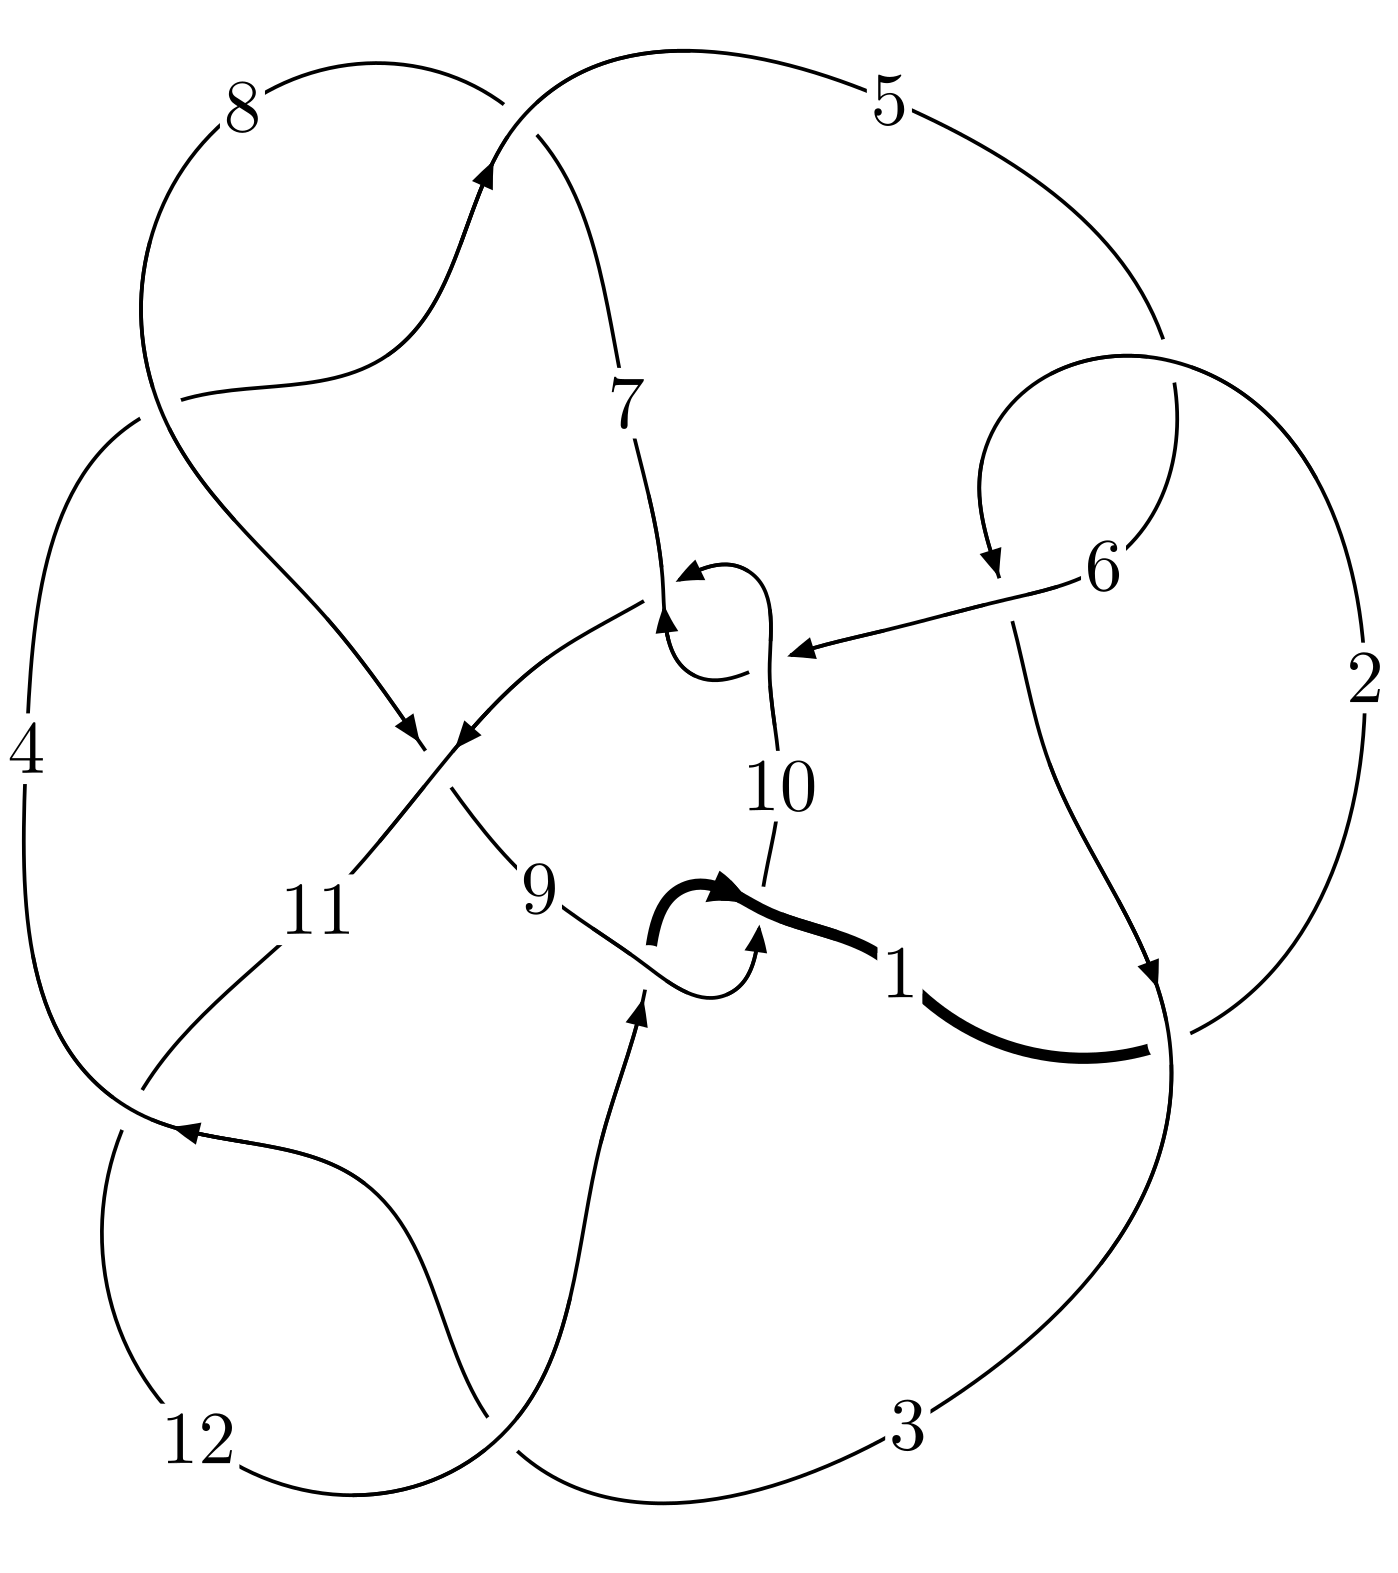
\includegraphics[width=112pt]{../../../GIT/diagram.site/Diagrams/png/1291_12a_0490.png}\\
\ \ \ A knot diagram\footnotemark}&
\allowdisplaybreaks
\textbf{Linearized knot diagam} \\
\cline{2-2}
 &
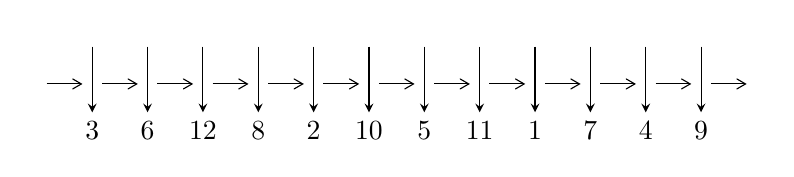
\begin{tikzpicture}[x=20pt, y=17pt]
	% nodes
	\node (C0) at (0, 0) {};
	\node (C1) at (1, 0) {};
	\node (C1U) at (1, +1) {};
	\node (C1D) at (1, -1) {3};

	\node (C2) at (2, 0) {};
	\node (C2U) at (2, +1) {};
	\node (C2D) at (2, -1) {6};

	\node (C3) at (3, 0) {};
	\node (C3U) at (3, +1) {};
	\node (C3D) at (3, -1) {12};

	\node (C4) at (4, 0) {};
	\node (C4U) at (4, +1) {};
	\node (C4D) at (4, -1) {8};

	\node (C5) at (5, 0) {};
	\node (C5U) at (5, +1) {};
	\node (C5D) at (5, -1) {2};

	\node (C6) at (6, 0) {};
	\node (C6U) at (6, +1) {};
	\node (C6D) at (6, -1) {10};

	\node (C7) at (7, 0) {};
	\node (C7U) at (7, +1) {};
	\node (C7D) at (7, -1) {5};

	\node (C8) at (8, 0) {};
	\node (C8U) at (8, +1) {};
	\node (C8D) at (8, -1) {11};

	\node (C9) at (9, 0) {};
	\node (C9U) at (9, +1) {};
	\node (C9D) at (9, -1) {1};

	\node (C10) at (10, 0) {};
	\node (C10U) at (10, +1) {};
	\node (C10D) at (10, -1) {7};

	\node (C11) at (11, 0) {};
	\node (C11U) at (11, +1) {};
	\node (C11D) at (11, -1) {4};

	\node (C12) at (12, 0) {};
	\node (C12U) at (12, +1) {};
	\node (C12D) at (12, -1) {9};
	\node (C13) at (13, 0) {};

	% arrows
	\draw[->,>={angle 60}]
	(C0) edge (C1) (C1) edge (C2) (C2) edge (C3) (C3) edge (C4) (C4) edge (C5) (C5) edge (C6) (C6) edge (C7) (C7) edge (C8) (C8) edge (C9) (C9) edge (C10) (C10) edge (C11) (C11) edge (C12) (C12) edge (C13) ;	\draw[->,>=stealth]
	(C1U) edge (C1D) (C2U) edge (C2D) (C3U) edge (C3D) (C4U) edge (C4D) (C5U) edge (C5D) (C6U) edge (C6D) (C7U) edge (C7D) (C8U) edge (C8D) (C9U) edge (C9D) (C10U) edge (C10D) (C11U) edge (C11D) (C12U) edge (C12D) ;
	\end{tikzpicture} \\
\hhline{~~} \\& 
\textbf{Solving Sequence} \\ \cline{2-2} 
 &
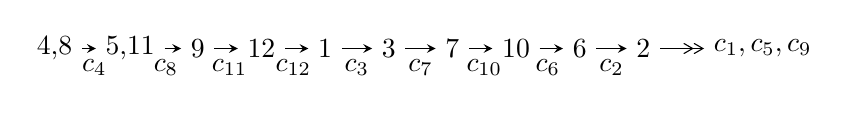
\begin{tikzpicture}[x=23pt, y=7pt]
	% node
	\node (A0) at (-1/8, 0) {4,8};
	\node (A1) at (17/16, 0) {5,11};
	\node (A2) at (17/8, 0) {9};
	\node (A3) at (25/8, 0) {12};
	\node (A4) at (33/8, 0) {1};
	\node (A5) at (41/8, 0) {3};
	\node (A6) at (49/8, 0) {7};
	\node (A7) at (57/8, 0) {10};
	\node (A8) at (65/8, 0) {6};
	\node (A9) at (73/8, 0) {2};
	\node (C1) at (1/2, -1) {$c_{4}$};
	\node (C2) at (13/8, -1) {$c_{8}$};
	\node (C3) at (21/8, -1) {$c_{11}$};
	\node (C4) at (29/8, -1) {$c_{12}$};
	\node (C5) at (37/8, -1) {$c_{3}$};
	\node (C6) at (45/8, -1) {$c_{7}$};
	\node (C7) at (53/8, -1) {$c_{10}$};
	\node (C8) at (61/8, -1) {$c_{6}$};
	\node (C9) at (69/8, -1) {$c_{2}$};
	\node (A10) at (11, 0) {$c_{1},c_{5},c_{9}$};

	% edge
	\draw[->,>=stealth]	
	(A0) edge (A1) (A1) edge (A2) (A2) edge (A3) (A3) edge (A4) (A4) edge (A5) (A5) edge (A6) (A6) edge (A7) (A7) edge (A8) (A8) edge (A9) ;
	\draw[->>,>={angle 60}]	
	(A9) edge (A10);
\end{tikzpicture} \\ 

\end{tabular} \\

\footnotetext{
The image of knot diagram is generated by the software ``\textbf{Draw programme}" developed by Andrew Bartholomew(\url{http://www.layer8.co.uk/maths/draw/index.htm\#Running-draw}), where we modified some parts for our purpose(\url{https://github.com/CATsTAILs/LinksPainter}).
}\phantom \\ \newline 
\centering \textbf{Ideals for irreducible components\footnotemark of $X_{\text{par}}$} 
 
\begin{align*}
I^u_{1}&=\langle 
b- u,\\
\phantom{I^u_{1}}&\phantom{= \langle  }250936582341786 u^{28}-122066524221929 u^{27}+\cdots+148804454046473 a-98424746117489,\\
\phantom{I^u_{1}}&\phantom{= \langle  }u^{29}- u^{28}+\cdots+2 u+1\rangle \\
I^u_{2}&=\langle 
-1.05564\times10^{344} u^{87}+9.79310\times10^{344} u^{86}+\cdots+1.52446\times10^{344} b+3.97004\times10^{347},\\
\phantom{I^u_{2}}&\phantom{= \langle  }-5.49731\times10^{346} u^{87}+3.25834\times10^{347} u^{86}+\cdots+1.25158\times10^{347} a+5.74130\times10^{349},\\
\phantom{I^u_{2}}&\phantom{= \langle  }u^{88}-5 u^{87}+\cdots+3584 u+821\rangle \\
I^u_{3}&=\langle 
b+u,\;- u^{11}+u^{10}-7 u^9+7 u^8-22 u^7+20 u^6-38 u^5+30 u^4-36 u^3+23 u^2+a-16 u+7,\\
\phantom{I^u_{3}}&\phantom{= \langle  }u^{14}- u^{13}+8 u^{12}-7 u^{11}+28 u^{10}-21 u^9+55 u^8-35 u^7+64 u^6-34 u^5+42 u^4-18 u^3+12 u^2-4 u-1\rangle \\
\\
\end{align*}
\raggedright * 3 irreducible components of $\dim_{\mathbb{C}}=0$, with total 131 representations.\\
\footnotetext{All coefficients of polynomials are rational numbers. But the coefficients are sometimes approximated in decimal forms when there is not enough margin.}
\newpage
\renewcommand{\arraystretch}{1}
\centering \section*{I. $I^u_{1}= \langle b- u,\;2.51\times10^{14} u^{28}-1.22\times10^{14} u^{27}+\cdots+1.49\times10^{14} a-9.84\times10^{13},\;u^{29}- u^{28}+\cdots+2 u+1 \rangle$}
\flushleft \textbf{(i) Arc colorings}\\
\begin{tabular}{m{7pt} m{180pt} m{7pt} m{180pt} }
\flushright $a_{4}=$&$\begin{pmatrix}1\\0\end{pmatrix}$ \\
\flushright $a_{8}=$&$\begin{pmatrix}0\\u\end{pmatrix}$ \\
\flushright $a_{5}=$&$\begin{pmatrix}1\\u^2\end{pmatrix}$ \\
\flushright $a_{11}=$&$\begin{pmatrix}-1.68635 u^{28}+0.820315 u^{27}+\cdots-0.162655 u+0.661437\\u\end{pmatrix}$ \\
\flushright $a_{9}=$&$\begin{pmatrix}2.67746 u^{28}-0.133672 u^{27}+\cdots-1.06713 u+0.714235\\-1.08667 u^{28}-0.0581082 u^{27}+\cdots-2.41842 u-0.866036\end{pmatrix}$ \\
\flushright $a_{12}=$&$\begin{pmatrix}-1.68635 u^{28}+0.820315 u^{27}+\cdots-1.16266 u+0.661437\\u\end{pmatrix}$ \\
\flushright $a_{1}=$&$\begin{pmatrix}2.38291 u^{28}+0.0817397 u^{27}+\cdots-2.92353 u+0.0907982\\-1.36536 u^{28}+0.339734 u^{27}+\cdots-2.62020 u-1.13818\end{pmatrix}$ \\
\flushright $a_{3}=$&$\begin{pmatrix}0.866036 u^{28}-1.95270 u^{27}+\cdots-4.03414 u-0.686351\\- u^2\end{pmatrix}$ \\
\flushright $a_{7}=$&$\begin{pmatrix}u\\u^3+u\end{pmatrix}$ \\
\flushright $a_{10}=$&$\begin{pmatrix}-1.40957 u^{28}+0.932959 u^{27}+\cdots-0.204858 u+0.940177\\0.250397 u^{28}-0.395790 u^{27}+\cdots-0.0978403 u-0.110687\end{pmatrix}$ \\
\flushright $a_{6}=$&$\begin{pmatrix}-1.70921 u^{28}+1.67866 u^{27}+\cdots+6.16797 u+1.12970\\-0.197996 u^{28}-0.326044 u^{27}+\cdots-1.09569 u-0.941452\end{pmatrix}$ \\
\flushright $a_{2}=$&$\begin{pmatrix}0.525755 u^{28}-0.0225068 u^{27}+\cdots-7.84043 u-1.04956\\-0.197996 u^{28}-0.326044 u^{27}+\cdots-1.09569 u-0.941452\end{pmatrix}$\\&\end{tabular}
\flushleft \textbf{(ii) Obstruction class $= -1$}\\~\\
\flushleft \textbf{(iii) Cusp Shapes $= \frac{566288427861444}{148804454046473} u^{28}-\frac{861558207456155}{148804454046473} u^{27}+\cdots-\frac{4146887141209843}{148804454046473} u-\frac{3721831975657214}{148804454046473}$}\\~\\
\newpage\renewcommand{\arraystretch}{1}
\flushleft \textbf{(iv) u-Polynomials at the component}\newline \\
\begin{tabular}{m{50pt}|m{274pt}}
Crossings & \hspace{64pt}u-Polynomials at each crossing \\
\hline $$\begin{aligned}c_{1}\end{aligned}$$&$\begin{aligned}
&u^{29}+11 u^{28}+\cdots+4736 u+256
\end{aligned}$\\
\hline $$\begin{aligned}c_{2},c_{5}\end{aligned}$$&$\begin{aligned}
&u^{29}+11 u^{28}+\cdots+192 u+16
\end{aligned}$\\
\hline $$\begin{aligned}c_{3},c_{4},c_{7}\\c_{11}\end{aligned}$$&$\begin{aligned}
&u^{29}- u^{28}+\cdots+2 u+1
\end{aligned}$\\
\hline $$\begin{aligned}c_{6},c_{9},c_{10}\\c_{12}\end{aligned}$$&$\begin{aligned}
&u^{29}- u^{28}+\cdots+4 u+1
\end{aligned}$\\
\hline $$\begin{aligned}c_{8}\end{aligned}$$&$\begin{aligned}
&u^{29}-28 u^{28}+\cdots-6144 u+2048
\end{aligned}$\\
\hline
\end{tabular}\\~\\
\newpage\renewcommand{\arraystretch}{1}
\flushleft \textbf{(v) Riley Polynomials at the component}\newline \\
\begin{tabular}{m{50pt}|m{274pt}}
Crossings & \hspace{64pt}Riley Polynomials at each crossing \\
\hline $$\begin{aligned}c_{1}\end{aligned}$$&$\begin{aligned}
&y^{29}+13 y^{28}+\cdots+9166848 y-65536
\end{aligned}$\\
\hline $$\begin{aligned}c_{2},c_{5}\end{aligned}$$&$\begin{aligned}
&y^{29}-11 y^{28}+\cdots+4736 y-256
\end{aligned}$\\
\hline $$\begin{aligned}c_{3},c_{4},c_{7}\\c_{11}\end{aligned}$$&$\begin{aligned}
&y^{29}+23 y^{28}+\cdots+20 y-1
\end{aligned}$\\
\hline $$\begin{aligned}c_{6},c_{9},c_{10}\\c_{12}\end{aligned}$$&$\begin{aligned}
&y^{29}-21 y^{28}+\cdots+16 y-1
\end{aligned}$\\
\hline $$\begin{aligned}c_{8}\end{aligned}$$&$\begin{aligned}
&y^{29}-4 y^{28}+\cdots-31457280 y-4194304
\end{aligned}$\\
\hline
\end{tabular}\\~\\
\newpage\flushleft \textbf{(vi) Complex Volumes and Cusp Shapes}
$$\begin{array}{c|c|c}  
\text{Solutions to }I^u_{1}& \I (\text{vol} + \sqrt{-1}CS) & \text{Cusp shape}\\
 \hline 
\begin{aligned}
u &= \phantom{-}0.943671 + 0.254326 I \\
a &= \phantom{-}1.002260 - 0.565360 I \\
b &= \phantom{-}0.943671 + 0.254326 I\end{aligned}
 & -6.98851 + 7.38189 I & -18.4807 - 4.8783 I \\ \hline\begin{aligned}
u &= \phantom{-}0.943671 - 0.254326 I \\
a &= \phantom{-}1.002260 + 0.565360 I \\
b &= \phantom{-}0.943671 - 0.254326 I\end{aligned}
 & -6.98851 - 7.38189 I & -18.4807 + 4.8783 I \\ \hline\begin{aligned}
u &= -0.931114 + 0.157675 I \\
a &= -1.095410 - 0.365233 I \\
b &= -0.931114 + 0.157675 I\end{aligned}
 & -5.01123 - 1.88675 I & -17.5811 + 0.8407 I \\ \hline\begin{aligned}
u &= -0.931114 - 0.157675 I \\
a &= -1.095410 + 0.365233 I \\
b &= -0.931114 - 0.157675 I\end{aligned}
 & -5.01123 + 1.88675 I & -17.5811 - 0.8407 I \\ \hline\begin{aligned}
u &= -0.382213 + 0.987155 I \\
a &= -0.742302 - 0.002124 I \\
b &= -0.382213 + 0.987155 I\end{aligned}
 & \phantom{-}1.88723 + 3.15225 I & -8.02900 - 4.43437 I \\ \hline\begin{aligned}
u &= -0.382213 - 0.987155 I \\
a &= -0.742302 + 0.002124 I \\
b &= -0.382213 - 0.987155 I\end{aligned}
 & \phantom{-}1.88723 - 3.15225 I & -8.02900 + 4.43437 I \\ \hline\begin{aligned}
u &= \phantom{-}0.048532 + 1.085820 I \\
a &= -2.00236 - 1.54010 I \\
b &= \phantom{-}0.048532 + 1.085820 I\end{aligned}
 & \phantom{-}0.49844 - 7.80036 I & -10.28673 + 6.90769 I \\ \hline\begin{aligned}
u &= \phantom{-}0.048532 - 1.085820 I \\
a &= -2.00236 + 1.54010 I \\
b &= \phantom{-}0.048532 - 1.085820 I\end{aligned}
 & \phantom{-}0.49844 + 7.80036 I & -10.28673 - 6.90769 I \\ \hline\begin{aligned}
u &= \phantom{-}0.080324 + 1.107540 I \\
a &= \phantom{-}1.71771 - 0.28078 I \\
b &= \phantom{-}0.080324 + 1.107540 I\end{aligned}
 & \phantom{-}4.67366 + 1.54454 I & -5.37934 - 3.77559 I \\ \hline\begin{aligned}
u &= \phantom{-}0.080324 - 1.107540 I \\
a &= \phantom{-}1.71771 + 0.28078 I \\
b &= \phantom{-}0.080324 - 1.107540 I\end{aligned}
 & \phantom{-}4.67366 - 1.54454 I & -5.37934 + 3.77559 I\\
 \hline 
 \end{array}$$\newpage$$\begin{array}{c|c|c}  
\text{Solutions to }I^u_{1}& \I (\text{vol} + \sqrt{-1}CS) & \text{Cusp shape}\\
 \hline 
\begin{aligned}
u &= \phantom{-}0.537814 + 0.473191 I \\
a &= \phantom{-}0.64181 + 1.26516 I \\
b &= \phantom{-}0.537814 + 0.473191 I\end{aligned}
 & -2.87090 + 3.41002 I & -17.4789 - 2.4204 I \\ \hline\begin{aligned}
u &= \phantom{-}0.537814 - 0.473191 I \\
a &= \phantom{-}0.64181 - 1.26516 I \\
b &= \phantom{-}0.537814 - 0.473191 I\end{aligned}
 & -2.87090 - 3.41002 I & -17.4789 + 2.4204 I \\ \hline\begin{aligned}
u &= \phantom{-}0.464520 + 1.279870 I \\
a &= \phantom{-}1.55204 - 0.50969 I \\
b &= \phantom{-}0.464520 + 1.279870 I\end{aligned}
 & -3.93836 - 8.89106 I & -15.2442 + 6.9531 I \\ \hline\begin{aligned}
u &= \phantom{-}0.464520 - 1.279870 I \\
a &= \phantom{-}1.55204 + 0.50969 I \\
b &= \phantom{-}0.464520 - 1.279870 I\end{aligned}
 & -3.93836 + 8.89106 I & -15.2442 - 6.9531 I \\ \hline\begin{aligned}
u &= -0.128639 + 1.359520 I \\
a &= -0.86220 - 2.02768 I \\
b &= -0.128639 + 1.359520 I\end{aligned}
 & \phantom{-}5.82172 + 4.48234 I & -14.8090 - 6.0213 I \\ \hline\begin{aligned}
u &= -0.128639 - 1.359520 I \\
a &= -0.86220 + 2.02768 I \\
b &= -0.128639 - 1.359520 I\end{aligned}
 & \phantom{-}5.82172 - 4.48234 I & -14.8090 + 6.0213 I \\ \hline\begin{aligned}
u &= \phantom{-}0.254997 + 1.384100 I \\
a &= \phantom{-}0.889760 - 0.491762 I \\
b &= \phantom{-}0.254997 + 1.384100 I\end{aligned}
 & \phantom{-}9.13257 - 0.76587 I & -4.66197 - 1.18942 I \\ \hline\begin{aligned}
u &= \phantom{-}0.254997 - 1.384100 I \\
a &= \phantom{-}0.889760 + 0.491762 I \\
b &= \phantom{-}0.254997 - 1.384100 I\end{aligned}
 & \phantom{-}9.13257 + 0.76587 I & -4.66197 + 1.18942 I \\ \hline\begin{aligned}
u &= -0.33115 + 1.41930 I \\
a &= -0.822163 - 0.477668 I \\
b &= -0.33115 + 1.41930 I\end{aligned}
 & \phantom{-}8.79150 + 6.45231 I & -4.82568 - 4.60766 I \\ \hline\begin{aligned}
u &= -0.33115 - 1.41930 I \\
a &= -0.822163 + 0.477668 I \\
b &= -0.33115 - 1.41930 I\end{aligned}
 & \phantom{-}8.79150 - 6.45231 I & -4.82568 + 4.60766 I\\
 \hline 
 \end{array}$$\newpage$$\begin{array}{c|c|c}  
\text{Solutions to }I^u_{1}& \I (\text{vol} + \sqrt{-1}CS) & \text{Cusp shape}\\
 \hline 
\begin{aligned}
u &= \phantom{-}0.497017 + 0.157040 I \\
a &= \phantom{-}2.59708 - 1.03005 I \\
b &= \phantom{-}0.497017 + 0.157040 I\end{aligned}
 & -10.64620 - 0.03192 I & -29.1555 + 7.5854 I \\ \hline\begin{aligned}
u &= \phantom{-}0.497017 - 0.157040 I \\
a &= \phantom{-}2.59708 + 1.03005 I \\
b &= \phantom{-}0.497017 - 0.157040 I\end{aligned}
 & -10.64620 + 0.03192 I & -29.1555 - 7.5854 I \\ \hline\begin{aligned}
u &= -0.51917 + 1.42010 I \\
a &= -1.160960 - 0.482236 I \\
b &= -0.51917 + 1.42010 I\end{aligned}
 & \phantom{-}3.16273 + 12.79870 I & -10.04451 - 6.89203 I \\ \hline\begin{aligned}
u &= -0.51917 - 1.42010 I \\
a &= -1.160960 + 0.482236 I \\
b &= -0.51917 - 1.42010 I\end{aligned}
 & \phantom{-}3.16273 - 12.79870 I & -10.04451 + 6.89203 I \\ \hline\begin{aligned}
u &= \phantom{-}0.57303 + 1.43212 I \\
a &= \phantom{-}1.124520 - 0.387229 I \\
b &= \phantom{-}0.57303 + 1.43212 I\end{aligned}
 & \phantom{-}0.7116 - 19.0153 I & -12.0000 + 9.9067 I \\ \hline\begin{aligned}
u &= \phantom{-}0.57303 - 1.43212 I \\
a &= \phantom{-}1.124520 + 0.387229 I \\
b &= \phantom{-}0.57303 - 1.43212 I\end{aligned}
 & \phantom{-}0.7116 + 19.0153 I & -12.0000 - 9.9067 I \\ \hline\begin{aligned}
u &= -0.441008 + 0.034064 I \\
a &= \phantom{-}0.225680 + 0.493763 I \\
b &= -0.441008 + 0.034064 I\end{aligned}
 & -0.743051 + 0.035864 I & -12.27916 + 0.21691 I \\ \hline\begin{aligned}
u &= -0.441008 - 0.034064 I \\
a &= \phantom{-}0.225680 - 0.493763 I \\
b &= -0.441008 - 0.034064 I\end{aligned}
 & -0.743051 - 0.035864 I & -12.27916 - 0.21691 I \\ \hline\begin{aligned}
u &= -0.333214\phantom{ +0.000000I} \\
a &= \phantom{-}0.869115\phantom{ +0.000000I} \\
b &= -0.333214\phantom{ +0.000000I}\end{aligned}
 & -0.737681\phantom{ +0.000000I} & -13.2750\phantom{ +0.000000I}\\
 \hline 
 \end{array}$$\newpage\newpage\renewcommand{\arraystretch}{1}
\centering \section*{II. $I^u_{2}= \langle -1.06\times10^{344} u^{87}+9.79\times10^{344} u^{86}+\cdots+1.52\times10^{344} b+3.97\times10^{347},\;-5.50\times10^{346} u^{87}+3.26\times10^{347} u^{86}+\cdots+1.25\times10^{347} a+5.74\times10^{349},\;u^{88}-5 u^{87}+\cdots+3584 u+821 \rangle$}
\flushleft \textbf{(i) Arc colorings}\\
\begin{tabular}{m{7pt} m{180pt} m{7pt} m{180pt} }
\flushright $a_{4}=$&$\begin{pmatrix}1\\0\end{pmatrix}$ \\
\flushright $a_{8}=$&$\begin{pmatrix}0\\u\end{pmatrix}$ \\
\flushright $a_{5}=$&$\begin{pmatrix}1\\u^2\end{pmatrix}$ \\
\flushright $a_{11}=$&$\begin{pmatrix}0.439229 u^{87}-2.60338 u^{86}+\cdots-1546.53 u-458.724\\0.692469 u^{87}-6.42398 u^{86}+\cdots-11147.5 u-2604.23\end{pmatrix}$ \\
\flushright $a_{9}=$&$\begin{pmatrix}-0.518913 u^{87}+1.96411 u^{86}+\cdots-2137.91 u-428.380\\0.867957 u^{87}-4.16018 u^{86}+\cdots+1075.10 u+82.6704\end{pmatrix}$ \\
\flushright $a_{12}=$&$\begin{pmatrix}-0.253240 u^{87}+3.82061 u^{86}+\cdots+9601.01 u+2145.50\\0.692469 u^{87}-6.42398 u^{86}+\cdots-11147.5 u-2604.23\end{pmatrix}$ \\
\flushright $a_{1}=$&$\begin{pmatrix}-0.0184597 u^{87}+2.48755 u^{86}+\cdots+9882.72 u+2145.17\\0.231469 u^{87}-3.79527 u^{86}+\cdots-10084.6 u-2265.64\end{pmatrix}$ \\
\flushright $a_{3}=$&$\begin{pmatrix}-12.5530 u^{87}+62.9597 u^{86}+\cdots-3353.00 u+1681.05\\12.4523 u^{87}-61.5883 u^{86}+\cdots+6410.79 u-966.838\end{pmatrix}$ \\
\flushright $a_{7}=$&$\begin{pmatrix}u\\u^3+u\end{pmatrix}$ \\
\flushright $a_{10}=$&$\begin{pmatrix}-0.564831 u^{87}+5.00806 u^{86}+\cdots+8142.29 u+1879.73\\1.00653 u^{87}-7.68993 u^{86}+\cdots-9921.01 u-2393.09\end{pmatrix}$ \\
\flushright $a_{6}=$&$\begin{pmatrix}-1.49311 u^{87}+18.0746 u^{86}+\cdots+41278.3 u+9450.89\\2.02163 u^{87}-20.5931 u^{86}+\cdots-40530.9 u-9364.41\end{pmatrix}$ \\
\flushright $a_{2}=$&$\begin{pmatrix}-6.88891 u^{87}+31.1111 u^{86}+\cdots-14992.8 u-1995.33\\7.09278 u^{87}-32.1612 u^{86}+\cdots+14767.1 u+1898.83\end{pmatrix}$\\&\end{tabular}
\flushleft \textbf{(ii) Obstruction class $= -1$}\\~\\
\flushleft \textbf{(iii) Cusp Shapes $= -27.8190 u^{87}+141.290 u^{86}+\cdots+723.380 u+5434.35$}\\~\\
\newpage\renewcommand{\arraystretch}{1}
\flushleft \textbf{(iv) u-Polynomials at the component}\newline \\
\begin{tabular}{m{50pt}|m{274pt}}
Crossings & \hspace{64pt}u-Polynomials at each crossing \\
\hline $$\begin{aligned}c_{1}\end{aligned}$$&$\begin{aligned}
&(u^{44}+20 u^{43}+\cdots-16 u+1)^{2}
\end{aligned}$\\
\hline $$\begin{aligned}c_{2},c_{5}\end{aligned}$$&$\begin{aligned}
&(u^{44}-4 u^{43}+\cdots-6 u+1)^{2}
\end{aligned}$\\
\hline $$\begin{aligned}c_{3},c_{4},c_{7}\\c_{11}\end{aligned}$$&$\begin{aligned}
&u^{88}-5 u^{87}+\cdots+3584 u+821
\end{aligned}$\\
\hline $$\begin{aligned}c_{6},c_{9},c_{10}\\c_{12}\end{aligned}$$&$\begin{aligned}
&u^{88}-7 u^{87}+\cdots+6072 u+2143
\end{aligned}$\\
\hline $$\begin{aligned}c_{8}\end{aligned}$$&$\begin{aligned}
&(u^{44}+13 u^{43}+\cdots+2 u+1)^{2}
\end{aligned}$\\
\hline
\end{tabular}\\~\\
\newpage\renewcommand{\arraystretch}{1}
\flushleft \textbf{(v) Riley Polynomials at the component}\newline \\
\begin{tabular}{m{50pt}|m{274pt}}
Crossings & \hspace{64pt}Riley Polynomials at each crossing \\
\hline $$\begin{aligned}c_{1}\end{aligned}$$&$\begin{aligned}
&(y^{44}+12 y^{43}+\cdots-304 y+1)^{2}
\end{aligned}$\\
\hline $$\begin{aligned}c_{2},c_{5}\end{aligned}$$&$\begin{aligned}
&(y^{44}-20 y^{43}+\cdots+16 y+1)^{2}
\end{aligned}$\\
\hline $$\begin{aligned}c_{3},c_{4},c_{7}\\c_{11}\end{aligned}$$&$\begin{aligned}
&y^{88}+63 y^{87}+\cdots+24336392 y+674041
\end{aligned}$\\
\hline $$\begin{aligned}c_{6},c_{9},c_{10}\\c_{12}\end{aligned}$$&$\begin{aligned}
&y^{88}-53 y^{87}+\cdots-51150136 y+4592449
\end{aligned}$\\
\hline $$\begin{aligned}c_{8}\end{aligned}$$&$\begin{aligned}
&(y^{44}+11 y^{43}+\cdots+18 y+1)^{2}
\end{aligned}$\\
\hline
\end{tabular}\\~\\
\newpage\flushleft \textbf{(vi) Complex Volumes and Cusp Shapes}
$$\begin{array}{c|c|c}  
\text{Solutions to }I^u_{2}& \I (\text{vol} + \sqrt{-1}CS) & \text{Cusp shape}\\
 \hline 
\begin{aligned}
u &= \phantom{-}0.395638 + 0.897674 I \\
a &= -0.966465 + 0.057775 I \\
b &= -0.889235 + 0.045072 I\end{aligned}
 & -1.85154 - 1.07596 I & \phantom{-0.000000 } 0 \\ \hline\begin{aligned}
u &= \phantom{-}0.395638 - 0.897674 I \\
a &= -0.966465 - 0.057775 I \\
b &= -0.889235 - 0.045072 I\end{aligned}
 & -1.85154 + 1.07596 I & \phantom{-0.000000 } 0 \\ \hline\begin{aligned}
u &= \phantom{-}0.073867 + 0.973400 I \\
a &= \phantom{-}0.201414 - 0.380588 I \\
b &= \phantom{-}1.09574 + 3.02407 I\end{aligned}
 & \phantom{-}0.24162 + 2.29469 I & \phantom{-0.000000 } 0 \\ \hline\begin{aligned}
u &= \phantom{-}0.073867 - 0.973400 I \\
a &= \phantom{-}0.201414 + 0.380588 I \\
b &= \phantom{-}1.09574 - 3.02407 I\end{aligned}
 & \phantom{-}0.24162 - 2.29469 I & \phantom{-0.000000 } 0 \\ \hline\begin{aligned}
u &= \phantom{-}0.073294 + 0.968958 I \\
a &= -0.480856 - 0.007306 I \\
b &= -1.96092 + 1.07676 I\end{aligned}
 & -0.04172 - 1.45400 I & \phantom{-0.000000 } 0 \\ \hline\begin{aligned}
u &= \phantom{-}0.073294 - 0.968958 I \\
a &= -0.480856 + 0.007306 I \\
b &= -1.96092 - 1.07676 I\end{aligned}
 & -0.04172 + 1.45400 I & \phantom{-0.000000 } 0 \\ \hline\begin{aligned}
u &= -0.038949 + 1.035690 I \\
a &= \phantom{-}0.343018 - 0.118947 I \\
b &= \phantom{-}2.59996 + 1.95864 I\end{aligned}
 & -0.35467 - 2.14659 I & \phantom{-0.000000 } 0 \\ \hline\begin{aligned}
u &= -0.038949 - 1.035690 I \\
a &= \phantom{-}0.343018 + 0.118947 I \\
b &= \phantom{-}2.59996 - 1.95864 I\end{aligned}
 & -0.35467 + 2.14659 I & \phantom{-0.000000 } 0 \\ \hline\begin{aligned}
u &= \phantom{-}0.955388 + 0.102547 I \\
a &= \phantom{-}0.855043 - 0.861822 I \\
b &= \phantom{-}0.405184 - 1.151540 I\end{aligned}
 & -7.65072 + 3.83591 I & \phantom{-0.000000 } 0 \\ \hline\begin{aligned}
u &= \phantom{-}0.955388 - 0.102547 I \\
a &= \phantom{-}0.855043 + 0.861822 I \\
b &= \phantom{-}0.405184 + 1.151540 I\end{aligned}
 & -7.65072 - 3.83591 I & \phantom{-0.000000 } 0\\
 \hline 
 \end{array}$$\newpage$$\begin{array}{c|c|c}  
\text{Solutions to }I^u_{2}& \I (\text{vol} + \sqrt{-1}CS) & \text{Cusp shape}\\
 \hline 
\begin{aligned}
u &= \phantom{-}0.834509 + 0.426099 I \\
a &= -0.262631 + 0.915377 I \\
b &= -0.240202 + 0.346289 I\end{aligned}
 & -2.67980 + 3.03789 I & \phantom{-0.000000 } 0 \\ \hline\begin{aligned}
u &= \phantom{-}0.834509 - 0.426099 I \\
a &= -0.262631 - 0.915377 I \\
b &= -0.240202 - 0.346289 I\end{aligned}
 & -2.67980 - 3.03789 I & \phantom{-0.000000 } 0 \\ \hline\begin{aligned}
u &= \phantom{-}0.050002 + 1.064780 I \\
a &= \phantom{-}0.65309 + 1.56196 I \\
b &= \phantom{-}0.03049 - 1.42468 I\end{aligned}
 & \phantom{-}3.12667 - 3.60717 I & \phantom{-0.000000 } 0 \\ \hline\begin{aligned}
u &= \phantom{-}0.050002 - 1.064780 I \\
a &= \phantom{-}0.65309 - 1.56196 I \\
b &= \phantom{-}0.03049 + 1.42468 I\end{aligned}
 & \phantom{-}3.12667 + 3.60717 I & \phantom{-0.000000 } 0 \\ \hline\begin{aligned}
u &= \phantom{-}0.055190 + 1.073230 I \\
a &= -1.52665 + 1.47024 I \\
b &= -0.213176 - 1.345590 I\end{aligned}
 & \phantom{-}4.81705 - 2.76241 I & \phantom{-0.000000 } 0 \\ \hline\begin{aligned}
u &= \phantom{-}0.055190 - 1.073230 I \\
a &= -1.52665 - 1.47024 I \\
b &= -0.213176 + 1.345590 I\end{aligned}
 & \phantom{-}4.81705 + 2.76241 I & \phantom{-0.000000 } 0 \\ \hline\begin{aligned}
u &= -0.889235 + 0.045072 I \\
a &= \phantom{-}0.439046 + 0.972185 I \\
b &= \phantom{-}0.395638 + 0.897674 I\end{aligned}
 & -1.85154 - 1.07596 I & \phantom{-0.000000 } 0 \\ \hline\begin{aligned}
u &= -0.889235 - 0.045072 I \\
a &= \phantom{-}0.439046 - 0.972185 I \\
b &= \phantom{-}0.395638 - 0.897674 I\end{aligned}
 & -1.85154 + 1.07596 I & \phantom{-0.000000 } 0 \\ \hline\begin{aligned}
u &= \phantom{-}0.647480 + 0.909082 I \\
a &= \phantom{-}0.024179 + 0.846346 I \\
b &= -0.199072 - 0.252945 I\end{aligned}
 & -2.15599 - 3.18535 I & \phantom{-0.000000 } 0 \\ \hline\begin{aligned}
u &= \phantom{-}0.647480 - 0.909082 I \\
a &= \phantom{-}0.024179 - 0.846346 I \\
b &= -0.199072 + 0.252945 I\end{aligned}
 & -2.15599 + 3.18535 I & \phantom{-0.000000 } 0\\
 \hline 
 \end{array}$$\newpage$$\begin{array}{c|c|c}  
\text{Solutions to }I^u_{2}& \I (\text{vol} + \sqrt{-1}CS) & \text{Cusp shape}\\
 \hline 
\begin{aligned}
u &= -0.178775 + 0.837971 I \\
a &= -0.319898 + 0.723642 I \\
b &= -0.592632 - 0.388560 I\end{aligned}
 & -0.386166 - 0.237422 I & \phantom{-0.000000 } 0 \\ \hline\begin{aligned}
u &= -0.178775 - 0.837971 I \\
a &= -0.319898 - 0.723642 I \\
b &= -0.592632 + 0.388560 I\end{aligned}
 & -0.386166 + 0.237422 I & \phantom{-0.000000 } 0 \\ \hline\begin{aligned}
u &= -0.328506 + 1.104140 I \\
a &= -0.095113 + 0.833518 I \\
b &= \phantom{-}0.015522 - 0.689347 I\end{aligned}
 & -0.747511 - 0.306015 I & \phantom{-0.000000 } 0 \\ \hline\begin{aligned}
u &= -0.328506 - 1.104140 I \\
a &= -0.095113 - 0.833518 I \\
b &= \phantom{-}0.015522 + 0.689347 I\end{aligned}
 & -0.747511 + 0.306015 I & \phantom{-0.000000 } 0 \\ \hline\begin{aligned}
u &= -0.100279 + 0.833670 I \\
a &= \phantom{-}2.36321 - 0.00085 I \\
b &= \phantom{-}0.447405 - 1.151160 I\end{aligned}
 & -0.63675 + 7.68993 I & \phantom{-0.000000 } 0 \\ \hline\begin{aligned}
u &= -0.100279 - 0.833670 I \\
a &= \phantom{-}2.36321 + 0.00085 I \\
b &= \phantom{-}0.447405 + 1.151160 I\end{aligned}
 & -0.63675 - 7.68993 I & \phantom{-0.000000 } 0 \\ \hline\begin{aligned}
u &= -1.153470 + 0.179310 I \\
a &= -0.747986 + 0.443896 I \\
b &= -0.486604 + 1.201200 I\end{aligned}
 & -1.78617 + 6.93892 I & \phantom{-0.000000 } 0 \\ \hline\begin{aligned}
u &= -1.153470 - 0.179310 I \\
a &= -0.747986 - 0.443896 I \\
b &= -0.486604 - 1.201200 I\end{aligned}
 & -1.78617 - 6.93892 I & \phantom{-0.000000 } 0 \\ \hline\begin{aligned}
u &= -0.701991 + 0.444562 I \\
a &= \phantom{-}1.17696 - 0.84810 I \\
b &= \phantom{-}0.516282 - 1.154410 I\end{aligned}
 & -0.31349 + 8.13644 I & \phantom{-0.000000 } 0 \\ \hline\begin{aligned}
u &= -0.701991 - 0.444562 I \\
a &= \phantom{-}1.17696 + 0.84810 I \\
b &= \phantom{-}0.516282 + 1.154410 I\end{aligned}
 & -0.31349 - 8.13644 I & \phantom{-0.000000 } 0\\
 \hline 
 \end{array}$$\newpage$$\begin{array}{c|c|c}  
\text{Solutions to }I^u_{2}& \I (\text{vol} + \sqrt{-1}CS) & \text{Cusp shape}\\
 \hline 
\begin{aligned}
u &= -0.024127 + 1.204100 I \\
a &= \phantom{-}0.686741 + 0.070014 I \\
b &= \phantom{-}0.304156 + 0.429506 I\end{aligned}
 & \phantom{-}3.28142 + 1.60364 I & \phantom{-0.000000 } 0 \\ \hline\begin{aligned}
u &= -0.024127 - 1.204100 I \\
a &= \phantom{-}0.686741 - 0.070014 I \\
b &= \phantom{-}0.304156 - 0.429506 I\end{aligned}
 & \phantom{-}3.28142 - 1.60364 I & \phantom{-0.000000 } 0 \\ \hline\begin{aligned}
u &= \phantom{-}0.405184 + 1.151540 I \\
a &= \phantom{-}0.814636 - 0.499504 I \\
b &= \phantom{-}0.955388 - 0.102547 I\end{aligned}
 & -7.65072 - 3.83591 I & \phantom{-0.000000 } 0 \\ \hline\begin{aligned}
u &= \phantom{-}0.405184 - 1.151540 I \\
a &= \phantom{-}0.814636 + 0.499504 I \\
b &= \phantom{-}0.955388 + 0.102547 I\end{aligned}
 & -7.65072 + 3.83591 I & \phantom{-0.000000 } 0 \\ \hline\begin{aligned}
u &= -0.383405 + 1.159460 I \\
a &= \phantom{-}0.861897 - 0.051187 I \\
b &= \phantom{-}0.508261 - 0.130931 I\end{aligned}
 & \phantom{-}2.08931 + 3.53746 I & \phantom{-0.000000 } 0 \\ \hline\begin{aligned}
u &= -0.383405 - 1.159460 I \\
a &= \phantom{-}0.861897 + 0.051187 I \\
b &= \phantom{-}0.508261 + 0.130931 I\end{aligned}
 & \phantom{-}2.08931 - 3.53746 I & \phantom{-0.000000 } 0 \\ \hline\begin{aligned}
u &= \phantom{-}0.447405 + 1.151160 I \\
a &= -1.55621 - 0.39958 I \\
b &= -0.100279 - 0.833670 I\end{aligned}
 & -0.63675 - 7.68993 I & \phantom{-0.000000 } 0 \\ \hline\begin{aligned}
u &= \phantom{-}0.447405 - 1.151160 I \\
a &= -1.55621 + 0.39958 I \\
b &= -0.100279 + 0.833670 I\end{aligned}
 & -0.63675 + 7.68993 I & \phantom{-0.000000 } 0 \\ \hline\begin{aligned}
u &= -0.333877 + 1.193500 I \\
a &= -0.578142 + 0.203628 I \\
b &= -0.095833 + 0.719086 I\end{aligned}
 & \phantom{-}2.00913 + 3.28257 I & \phantom{-0.000000 } 0 \\ \hline\begin{aligned}
u &= -0.333877 - 1.193500 I \\
a &= -0.578142 - 0.203628 I \\
b &= -0.095833 - 0.719086 I\end{aligned}
 & \phantom{-}2.00913 - 3.28257 I & \phantom{-0.000000 } 0\\
 \hline 
 \end{array}$$\newpage$$\begin{array}{c|c|c}  
\text{Solutions to }I^u_{2}& \I (\text{vol} + \sqrt{-1}CS) & \text{Cusp shape}\\
 \hline 
\begin{aligned}
u &= \phantom{-}0.516282 + 1.154410 I \\
a &= -0.952479 - 0.036873 I \\
b &= -0.701991 - 0.444562 I\end{aligned}
 & -0.31349 - 8.13644 I & \phantom{-0.000000 } 0 \\ \hline\begin{aligned}
u &= \phantom{-}0.516282 - 1.154410 I \\
a &= -0.952479 + 0.036873 I \\
b &= -0.701991 + 0.444562 I\end{aligned}
 & -0.31349 + 8.13644 I & \phantom{-0.000000 } 0 \\ \hline\begin{aligned}
u &= -0.095833 + 0.719086 I \\
a &= -1.026620 + 0.206353 I \\
b &= -0.333877 + 1.193500 I\end{aligned}
 & \phantom{-}2.00913 + 3.28257 I & -12.00000 + 0. I\phantom{ +0.000000I} \\ \hline\begin{aligned}
u &= -0.095833 - 0.719086 I \\
a &= -1.026620 - 0.206353 I \\
b &= -0.333877 - 1.193500 I\end{aligned}
 & \phantom{-}2.00913 - 3.28257 I & -12.00000 + 0. I\phantom{ +0.000000I} \\ \hline\begin{aligned}
u &= \phantom{-}0.510456 + 1.178910 I \\
a &= \phantom{-}0.717263 - 0.320490 I \\
b &= \phantom{-}1.301060 + 0.116336 I\end{aligned}
 & -4.09684 - 12.57490 I & \phantom{-0.000000 } 0 \\ \hline\begin{aligned}
u &= \phantom{-}0.510456 - 1.178910 I \\
a &= \phantom{-}0.717263 + 0.320490 I \\
b &= \phantom{-}1.301060 - 0.116336 I\end{aligned}
 & -4.09684 + 12.57490 I & \phantom{-0.000000 } 0 \\ \hline\begin{aligned}
u &= -0.592632 + 0.388560 I \\
a &= \phantom{-}0.955615 - 0.044076 I \\
b &= -0.178775 - 0.837971 I\end{aligned}
 & -0.386166 + 0.237422 I & -12.00000 + 0. I\phantom{ +0.000000I} \\ \hline\begin{aligned}
u &= -0.592632 - 0.388560 I \\
a &= \phantom{-}0.955615 + 0.044076 I \\
b &= -0.178775 + 0.837971 I\end{aligned}
 & -0.386166 - 0.237422 I & -12.00000 + 0. I\phantom{ +0.000000I} \\ \hline\begin{aligned}
u &= -0.486604 + 1.201200 I \\
a &= -0.688975 - 0.372898 I \\
b &= -1.153470 + 0.179310 I\end{aligned}
 & -1.78617 + 6.93892 I & \phantom{-0.000000 } 0 \\ \hline\begin{aligned}
u &= -0.486604 - 1.201200 I \\
a &= -0.688975 + 0.372898 I \\
b &= -1.153470 - 0.179310 I\end{aligned}
 & -1.78617 - 6.93892 I & \phantom{-0.000000 } 0\\
 \hline 
 \end{array}$$\newpage$$\begin{array}{c|c|c}  
\text{Solutions to }I^u_{2}& \I (\text{vol} + \sqrt{-1}CS) & \text{Cusp shape}\\
 \hline 
\begin{aligned}
u &= \phantom{-}1.301060 + 0.116336 I \\
a &= \phantom{-}0.613773 + 0.469300 I \\
b &= \phantom{-}0.510456 + 1.178910 I\end{aligned}
 & -4.09684 - 12.57490 I & \phantom{-0.000000 } 0 \\ \hline\begin{aligned}
u &= \phantom{-}1.301060 - 0.116336 I \\
a &= \phantom{-}0.613773 - 0.469300 I \\
b &= \phantom{-}0.510456 - 1.178910 I\end{aligned}
 & -4.09684 + 12.57490 I & \phantom{-0.000000 } 0 \\ \hline\begin{aligned}
u &= \phantom{-}0.015522 + 0.689347 I \\
a &= \phantom{-}0.520249 + 1.301450 I \\
b &= -0.328506 - 1.104140 I\end{aligned}
 & -0.747511 + 0.306015 I & -12.00000 + 0. I\phantom{ +0.000000I} \\ \hline\begin{aligned}
u &= \phantom{-}0.015522 - 0.689347 I \\
a &= \phantom{-}0.520249 - 1.301450 I \\
b &= -0.328506 + 1.104140 I\end{aligned}
 & -0.747511 - 0.306015 I & -12.00000 + 0. I\phantom{ +0.000000I} \\ \hline\begin{aligned}
u &= \phantom{-}0.285680 + 1.286210 I \\
a &= -1.097630 + 0.495754 I \\
b &= -0.56605 - 1.46741 I\end{aligned}
 & \phantom{-}6.43432 - 6.56301 I & \phantom{-0.000000 } 0 \\ \hline\begin{aligned}
u &= \phantom{-}0.285680 - 1.286210 I \\
a &= -1.097630 - 0.495754 I \\
b &= -0.56605 + 1.46741 I\end{aligned}
 & \phantom{-}6.43432 + 6.56301 I & \phantom{-0.000000 } 0 \\ \hline\begin{aligned}
u &= -0.213176 + 1.345590 I \\
a &= \phantom{-}1.31992 + 1.02616 I \\
b &= \phantom{-}0.055190 - 1.073230 I\end{aligned}
 & \phantom{-}4.81705 + 2.76241 I & \phantom{-0.000000 } 0 \\ \hline\begin{aligned}
u &= -0.213176 - 1.345590 I \\
a &= \phantom{-}1.31992 - 1.02616 I \\
b &= \phantom{-}0.055190 + 1.073230 I\end{aligned}
 & \phantom{-}4.81705 - 2.76241 I & \phantom{-0.000000 } 0 \\ \hline\begin{aligned}
u &= -0.491215 + 1.284550 I \\
a &= \phantom{-}1.058670 + 0.203604 I \\
b &= \phantom{-}0.680102 - 1.206280 I\end{aligned}
 & \phantom{-}1.92815 + 6.09693 I & \phantom{-0.000000 } 0 \\ \hline\begin{aligned}
u &= -0.491215 - 1.284550 I \\
a &= \phantom{-}1.058670 - 0.203604 I \\
b &= \phantom{-}0.680102 + 1.206280 I\end{aligned}
 & \phantom{-}1.92815 - 6.09693 I & \phantom{-0.000000 } 0\\
 \hline 
 \end{array}$$\newpage$$\begin{array}{c|c|c}  
\text{Solutions to }I^u_{2}& \I (\text{vol} + \sqrt{-1}CS) & \text{Cusp shape}\\
 \hline 
\begin{aligned}
u &= \phantom{-}0.680102 + 1.206280 I \\
a &= -1.069720 + 0.044812 I \\
b &= -0.491215 - 1.284550 I\end{aligned}
 & \phantom{-}1.92815 - 6.09693 I & \phantom{-0.000000 } 0 \\ \hline\begin{aligned}
u &= \phantom{-}0.680102 - 1.206280 I \\
a &= -1.069720 - 0.044812 I \\
b &= -0.491215 + 1.284550 I\end{aligned}
 & \phantom{-}1.92815 + 6.09693 I & \phantom{-0.000000 } 0 \\ \hline\begin{aligned}
u &= -0.328429 + 1.350810 I \\
a &= \phantom{-}1.008230 + 0.432064 I \\
b &= \phantom{-}0.66120 - 1.48553 I\end{aligned}
 & \phantom{-}4.98438 + 11.81130 I & \phantom{-0.000000 } 0 \\ \hline\begin{aligned}
u &= -0.328429 - 1.350810 I \\
a &= \phantom{-}1.008230 - 0.432064 I \\
b &= \phantom{-}0.66120 + 1.48553 I\end{aligned}
 & \phantom{-}4.98438 - 11.81130 I & \phantom{-0.000000 } 0 \\ \hline\begin{aligned}
u &= \phantom{-}0.03049 + 1.42468 I \\
a &= -0.567160 + 1.132320 I \\
b &= \phantom{-}0.050002 - 1.064780 I\end{aligned}
 & \phantom{-}3.12667 + 3.60717 I & \phantom{-0.000000 } 0 \\ \hline\begin{aligned}
u &= \phantom{-}0.03049 - 1.42468 I \\
a &= -0.567160 - 1.132320 I \\
b &= \phantom{-}0.050002 + 1.064780 I\end{aligned}
 & \phantom{-}3.12667 - 3.60717 I & \phantom{-0.000000 } 0 \\ \hline\begin{aligned}
u &= -0.326282 + 0.449657 I \\
a &= -1.29823 - 1.02321 I \\
b &= -0.31384 + 1.56248 I\end{aligned}
 & \phantom{-}0.36905 + 2.88717 I & -18.5219 - 5.6422 I \\ \hline\begin{aligned}
u &= -0.326282 - 0.449657 I \\
a &= -1.29823 + 1.02321 I \\
b &= -0.31384 - 1.56248 I\end{aligned}
 & \phantom{-}0.36905 - 2.88717 I & -18.5219 + 5.6422 I \\ \hline\begin{aligned}
u &= \phantom{-}0.304156 + 0.429506 I \\
a &= \phantom{-}1.16885 + 1.06258 I \\
b &= -0.024127 + 1.204100 I\end{aligned}
 & \phantom{-}3.28142 + 1.60364 I & -4.45910 - 2.86227 I \\ \hline\begin{aligned}
u &= \phantom{-}0.304156 - 0.429506 I \\
a &= \phantom{-}1.16885 - 1.06258 I \\
b &= -0.024127 - 1.204100 I\end{aligned}
 & \phantom{-}3.28142 - 1.60364 I & -4.45910 + 2.86227 I\\
 \hline 
 \end{array}$$\newpage$$\begin{array}{c|c|c}  
\text{Solutions to }I^u_{2}& \I (\text{vol} + \sqrt{-1}CS) & \text{Cusp shape}\\
 \hline 
\begin{aligned}
u &= \phantom{-}0.508261 + 0.130931 I \\
a &= -0.98451 - 1.75118 I \\
b &= -0.383405 - 1.159460 I\end{aligned}
 & \phantom{-}2.08931 - 3.53746 I & -7.63620 + 3.64913 I \\ \hline\begin{aligned}
u &= \phantom{-}0.508261 - 0.130931 I \\
a &= -0.98451 + 1.75118 I \\
b &= -0.383405 + 1.159460 I\end{aligned}
 & \phantom{-}2.08931 + 3.53746 I & -7.63620 - 3.64913 I \\ \hline\begin{aligned}
u &= -0.56605 + 1.46741 I \\
a &= \phantom{-}0.971128 + 0.273618 I \\
b &= \phantom{-}0.285680 - 1.286210 I\end{aligned}
 & \phantom{-}6.43432 + 6.56301 I & \phantom{-0.000000 } 0 \\ \hline\begin{aligned}
u &= -0.56605 - 1.46741 I \\
a &= \phantom{-}0.971128 - 0.273618 I \\
b &= \phantom{-}0.285680 + 1.286210 I\end{aligned}
 & \phantom{-}6.43432 - 6.56301 I & \phantom{-0.000000 } 0 \\ \hline\begin{aligned}
u &= -0.240202 + 0.346289 I \\
a &= \phantom{-}2.09505 + 0.30603 I \\
b &= \phantom{-}0.834509 + 0.426099 I\end{aligned}
 & -2.67980 + 3.03789 I & -17.8249 - 5.9672 I \\ \hline\begin{aligned}
u &= -0.240202 - 0.346289 I \\
a &= \phantom{-}2.09505 - 0.30603 I \\
b &= \phantom{-}0.834509 - 0.426099 I\end{aligned}
 & -2.67980 - 3.03789 I & -17.8249 + 5.9672 I \\ \hline\begin{aligned}
u &= -0.31384 + 1.56248 I \\
a &= -0.262929 - 0.512752 I \\
b &= -0.326282 + 0.449657 I\end{aligned}
 & \phantom{-}0.36905 + 2.88717 I & \phantom{-0.000000 } 0 \\ \hline\begin{aligned}
u &= -0.31384 - 1.56248 I \\
a &= -0.262929 + 0.512752 I \\
b &= -0.326282 - 0.449657 I\end{aligned}
 & \phantom{-}0.36905 - 2.88717 I & \phantom{-0.000000 } 0 \\ \hline\begin{aligned}
u &= \phantom{-}0.66120 + 1.48553 I \\
a &= -0.914234 + 0.208865 I \\
b &= -0.328429 - 1.350810 I\end{aligned}
 & \phantom{-}4.98438 - 11.81130 I & \phantom{-0.000000 } 0 \\ \hline\begin{aligned}
u &= \phantom{-}0.66120 - 1.48553 I \\
a &= -0.914234 - 0.208865 I \\
b &= -0.328429 + 1.350810 I\end{aligned}
 & \phantom{-}4.98438 + 11.81130 I & \phantom{-0.000000 } 0\\
 \hline 
 \end{array}$$\newpage$$\begin{array}{c|c|c}  
\text{Solutions to }I^u_{2}& \I (\text{vol} + \sqrt{-1}CS) & \text{Cusp shape}\\
 \hline 
\begin{aligned}
u &= -0.199072 + 0.252945 I \\
a &= \phantom{-}0.05673 + 2.93523 I \\
b &= \phantom{-}0.647480 - 0.909082 I\end{aligned}
 & -2.15599 + 3.18535 I & -16.4226 - 4.3884 I \\ \hline\begin{aligned}
u &= -0.199072 - 0.252945 I \\
a &= \phantom{-}0.05673 - 2.93523 I \\
b &= \phantom{-}0.647480 + 0.909082 I\end{aligned}
 & -2.15599 - 3.18535 I & -16.4226 + 4.3884 I \\ \hline\begin{aligned}
u &= -1.96092 + 1.07676 I \\
a &= -0.089326 + 0.188830 I \\
b &= \phantom{-}0.073294 + 0.968958 I\end{aligned}
 & -0.04172 - 1.45400 I & \phantom{-0.000000 } 0 \\ \hline\begin{aligned}
u &= -1.96092 - 1.07676 I \\
a &= -0.089326 - 0.188830 I \\
b &= \phantom{-}0.073294 - 0.968958 I\end{aligned}
 & -0.04172 + 1.45400 I & \phantom{-0.000000 } 0 \\ \hline\begin{aligned}
u &= \phantom{-}1.09574 + 3.02407 I \\
a &= \phantom{-}0.0899031 - 0.0948497 I \\
b &= \phantom{-}0.073867 + 0.973400 I\end{aligned}
 & \phantom{-}0.24162 + 2.29469 I & \phantom{-0.000000 } 0 \\ \hline\begin{aligned}
u &= \phantom{-}1.09574 - 3.02407 I \\
a &= \phantom{-}0.0899031 + 0.0948497 I \\
b &= \phantom{-}0.073867 - 0.973400 I\end{aligned}
 & \phantom{-}0.24162 - 2.29469 I & \phantom{-0.000000 } 0 \\ \hline\begin{aligned}
u &= \phantom{-}2.59996 + 1.95864 I \\
a &= \phantom{-}0.0934743 + 0.0680048 I \\
b &= -0.038949 + 1.035690 I\end{aligned}
 & -0.35467 - 2.14659 I & \phantom{-0.000000 } 0 \\ \hline\begin{aligned}
u &= \phantom{-}2.59996 - 1.95864 I \\
a &= \phantom{-}0.0934743 - 0.0680048 I \\
b &= -0.038949 - 1.035690 I\end{aligned}
 & -0.35467 + 2.14659 I & \phantom{-0.000000 } 0\\
 \hline 
 \end{array}$$\newpage\newpage\renewcommand{\arraystretch}{1}
\centering \section*{III. $I^u_{3}= \langle b+u,\;- u^{11}+u^{10}+\cdots+a+7,\;u^{14}- u^{13}+\cdots-4 u-1 \rangle$}
\flushleft \textbf{(i) Arc colorings}\\
\begin{tabular}{m{7pt} m{180pt} m{7pt} m{180pt} }
\flushright $a_{4}=$&$\begin{pmatrix}1\\0\end{pmatrix}$ \\
\flushright $a_{8}=$&$\begin{pmatrix}0\\u\end{pmatrix}$ \\
\flushright $a_{5}=$&$\begin{pmatrix}1\\u^2\end{pmatrix}$ \\
\flushright $a_{11}=$&$\begin{pmatrix}u^{11}- u^{10}+\cdots+16 u-7\\- u\end{pmatrix}$ \\
\flushright $a_{9}=$&$\begin{pmatrix}-4 u^{13}+4 u^{12}+\cdots-24 u+11\\u^{13}- u^{12}+\cdots-7 u^2+u\end{pmatrix}$ \\
\flushright $a_{12}=$&$\begin{pmatrix}u^{11}- u^{10}+\cdots+17 u-7\\- u\end{pmatrix}$ \\
\flushright $a_{1}=$&$\begin{pmatrix}-4 u^{13}+4 u^{12}+\cdots-23 u+11\\u^{13}-2 u^{12}+\cdots-10 u^2+u\end{pmatrix}$ \\
\flushright $a_{3}=$&$\begin{pmatrix}u^{12}- u^{11}+\cdots-7 u+1\\- u^2\end{pmatrix}$ \\
\flushright $a_{7}=$&$\begin{pmatrix}u\\u^3+u\end{pmatrix}$ \\
\flushright $a_{10}=$&$\begin{pmatrix}u^{12}+5 u^{10}+\cdots+15 u-7\\- u^{12}+u^{11}+\cdots+2 u+1\end{pmatrix}$ \\
\flushright $a_{6}=$&$\begin{pmatrix}u^{13}-2 u^{12}+\cdots+31 u-10\\u^{12}- u^{11}+\cdots+7 u^2-2 u\end{pmatrix}$ \\
\flushright $a_{2}=$&$\begin{pmatrix}-2 u^{13}+3 u^{12}+\cdots-30 u+12\\- u^{12}+u^{11}+\cdots-7 u^2+2 u\end{pmatrix}$\\&\end{tabular}
\flushleft \textbf{(ii) Obstruction class $= 1$}\\~\\
\flushleft \textbf{(iii) Cusp Shapes $= -4 u^{13}- u^{12}-28 u^{11}-7 u^{10}-82 u^9-27 u^8-130 u^7-53 u^6-119 u^5-45 u^4-66 u^3-5 u^2-23 u+6$}\\~\\
\newpage\renewcommand{\arraystretch}{1}
\flushleft \textbf{(iv) u-Polynomials at the component}\newline \\
\begin{tabular}{m{50pt}|m{274pt}}
Crossings & \hspace{64pt}u-Polynomials at each crossing \\
\hline $$\begin{aligned}c_{1}\end{aligned}$$&$\begin{aligned}
&u^{14}-6 u^{13}+\cdots-13 u+1
\end{aligned}$\\
\hline $$\begin{aligned}c_{2}\end{aligned}$$&$\begin{aligned}
&u^{14}+2 u^{13}+\cdots+3 u+1
\end{aligned}$\\
\hline $$\begin{aligned}c_{3},c_{7}\end{aligned}$$&$\begin{aligned}
&u^{14}+u^{13}+\cdots+4 u-1
\end{aligned}$\\
\hline $$\begin{aligned}c_{4},c_{11}\end{aligned}$$&$\begin{aligned}
&u^{14}- u^{13}+\cdots-4 u-1
\end{aligned}$\\
\hline $$\begin{aligned}c_{5}\end{aligned}$$&$\begin{aligned}
&u^{14}-2 u^{13}+\cdots-3 u+1
\end{aligned}$\\
\hline $$\begin{aligned}c_{6},c_{9}\end{aligned}$$&$\begin{aligned}
&u^{14}- u^{13}+\cdots+6 u^2-1
\end{aligned}$\\
\hline $$\begin{aligned}c_{8}\end{aligned}$$&$\begin{aligned}
&u^{14}-9 u^{13}+\cdots+15 u-1
\end{aligned}$\\
\hline $$\begin{aligned}c_{10},c_{12}\end{aligned}$$&$\begin{aligned}
&u^{14}+u^{13}+\cdots+6 u^2-1
\end{aligned}$\\
\hline
\end{tabular}\\~\\
\newpage\renewcommand{\arraystretch}{1}
\flushleft \textbf{(v) Riley Polynomials at the component}\newline \\
\begin{tabular}{m{50pt}|m{274pt}}
Crossings & \hspace{64pt}Riley Polynomials at each crossing \\
\hline $$\begin{aligned}c_{1}\end{aligned}$$&$\begin{aligned}
&y^{14}+10 y^{13}+\cdots-21 y+1
\end{aligned}$\\
\hline $$\begin{aligned}c_{2},c_{5}\end{aligned}$$&$\begin{aligned}
&y^{14}-6 y^{13}+\cdots-13 y+1
\end{aligned}$\\
\hline $$\begin{aligned}c_{3},c_{4},c_{7}\\c_{11}\end{aligned}$$&$\begin{aligned}
&y^{14}+15 y^{13}+\cdots-40 y+1
\end{aligned}$\\
\hline $$\begin{aligned}c_{6},c_{9},c_{10}\\c_{12}\end{aligned}$$&$\begin{aligned}
&y^{14}-13 y^{13}+\cdots-12 y+1
\end{aligned}$\\
\hline $$\begin{aligned}c_{8}\end{aligned}$$&$\begin{aligned}
&y^{14}-5 y^{13}+\cdots-29 y+1
\end{aligned}$\\
\hline
\end{tabular}\\~\\
\newpage\flushleft \textbf{(vi) Complex Volumes and Cusp Shapes}
$$\begin{array}{c|c|c}  
\text{Solutions to }I^u_{3}& \I (\text{vol} + \sqrt{-1}CS) & \text{Cusp shape}\\
 \hline 
\begin{aligned}
u &= \phantom{-}0.494303 + 0.948206 I \\
a &= -0.338246 + 0.404754 I \\
b &= -0.494303 - 0.948206 I\end{aligned}
 & \phantom{-}1.02409 - 2.16166 I & -11.75755 + 0.70501 I \\ \hline\begin{aligned}
u &= \phantom{-}0.494303 - 0.948206 I \\
a &= -0.338246 - 0.404754 I \\
b &= -0.494303 + 0.948206 I\end{aligned}
 & \phantom{-}1.02409 + 2.16166 I & -11.75755 - 0.70501 I \\ \hline\begin{aligned}
u &= -0.403796 + 1.012310 I \\
a &= \phantom{-}1.96277 - 0.70590 I \\
b &= \phantom{-}0.403796 - 1.012310 I\end{aligned}
 & -0.83998 + 9.12624 I & -13.7432 - 11.8895 I \\ \hline\begin{aligned}
u &= -0.403796 - 1.012310 I \\
a &= \phantom{-}1.96277 + 0.70590 I \\
b &= \phantom{-}0.403796 + 1.012310 I\end{aligned}
 & -0.83998 - 9.12624 I & -13.7432 + 11.8895 I \\ \hline\begin{aligned}
u &= -0.385160 + 1.187760 I \\
a &= \phantom{-}0.204583 + 0.322059 I \\
b &= \phantom{-}0.385160 - 1.187760 I\end{aligned}
 & \phantom{-}0.46872 - 2.66919 I & -10.42920 + 4.04963 I \\ \hline\begin{aligned}
u &= -0.385160 - 1.187760 I \\
a &= \phantom{-}0.204583 - 0.322059 I \\
b &= \phantom{-}0.385160 + 1.187760 I\end{aligned}
 & \phantom{-}0.46872 + 2.66919 I & -10.42920 - 4.04963 I \\ \hline\begin{aligned}
u &= \phantom{-}0.141069 + 1.315050 I \\
a &= -1.06420 + 2.01626 I \\
b &= -0.141069 - 1.315050 I\end{aligned}
 & \phantom{-}6.31414 - 4.36226 I & \phantom{-}1.13088 + 3.35215 I \\ \hline\begin{aligned}
u &= \phantom{-}0.141069 - 1.315050 I \\
a &= -1.06420 - 2.01626 I \\
b &= -0.141069 + 1.315050 I\end{aligned}
 & \phantom{-}6.31414 + 4.36226 I & \phantom{-}1.13088 - 3.35215 I \\ \hline\begin{aligned}
u &= \phantom{-}0.569251 + 1.216470 I \\
a &= -1.045770 + 0.078978 I \\
b &= -0.569251 - 1.216470 I\end{aligned}
 & \phantom{-}3.10148 - 6.42639 I & -6.16249 + 6.22632 I \\ \hline\begin{aligned}
u &= \phantom{-}0.569251 - 1.216470 I \\
a &= -1.045770 - 0.078978 I \\
b &= -0.569251 + 1.216470 I\end{aligned}
 & \phantom{-}3.10148 + 6.42639 I & -6.16249 - 6.22632 I\\
 \hline 
 \end{array}$$\newpage$$\begin{array}{c|c|c}  
\text{Solutions to }I^u_{3}& \I (\text{vol} + \sqrt{-1}CS) & \text{Cusp shape}\\
 \hline 
\begin{aligned}
u &= -0.080538 + 1.411260 I \\
a &= \phantom{-}0.032468 + 0.269326 I \\
b &= \phantom{-}0.080538 - 1.411260 I\end{aligned}
 & -0.61736 + 1.76932 I & -9.28138 - 4.00219 I \\ \hline\begin{aligned}
u &= -0.080538 - 1.411260 I \\
a &= \phantom{-}0.032468 - 0.269326 I \\
b &= \phantom{-}0.080538 + 1.411260 I\end{aligned}
 & -0.61736 - 1.76932 I & -9.28138 + 4.00219 I \\ \hline\begin{aligned}
u &= \phantom{-}0.484377\phantom{ +0.000000I} \\
a &= -1.32520\phantom{ +0.000000I} \\
b &= -0.484377\phantom{ +0.000000I}\end{aligned}
 & -1.88989\phantom{ +0.000000I} & -21.1800\phantom{ +0.000000I} \\ \hline\begin{aligned}
u &= -0.154632\phantom{ +0.000000I} \\
a &= -10.1780\phantom{ +0.000000I} \\
b &= \phantom{-}0.154632\phantom{ +0.000000I}\end{aligned}
 & -10.4326\phantom{ +0.000000I} & \phantom{-}9.66530\phantom{ +0.000000I}\\
 \hline 
 \end{array}$$\newpage
\newpage\renewcommand{\arraystretch}{1}
\centering \section*{ IV. u-Polynomials}
\begin{tabular}{m{50pt}|m{274pt}}
Crossings & \hspace{64pt}u-Polynomials at each crossing \\
\hline $$\begin{aligned}c_{1}\end{aligned}$$&$\begin{aligned}
&(u^{14}-6 u^{13}+\cdots-13 u+1)(u^{29}+11 u^{28}+\cdots+4736 u+256)\\
&\cdot(u^{44}+20 u^{43}+\cdots-16 u+1)^{2}
\end{aligned}$\\
\hline $$\begin{aligned}c_{2}\end{aligned}$$&$\begin{aligned}
&(u^{14}+2 u^{13}+\cdots+3 u+1)(u^{29}+11 u^{28}+\cdots+192 u+16)\\
&\cdot(u^{44}-4 u^{43}+\cdots-6 u+1)^{2}
\end{aligned}$\\
\hline $$\begin{aligned}c_{3},c_{7}\end{aligned}$$&$\begin{aligned}
&(u^{14}+u^{13}+\cdots+4 u-1)(u^{29}- u^{28}+\cdots+2 u+1)\\
&\cdot(u^{88}-5 u^{87}+\cdots+3584 u+821)
\end{aligned}$\\
\hline $$\begin{aligned}c_{4},c_{11}\end{aligned}$$&$\begin{aligned}
&(u^{14}- u^{13}+\cdots-4 u-1)(u^{29}- u^{28}+\cdots+2 u+1)\\
&\cdot(u^{88}-5 u^{87}+\cdots+3584 u+821)
\end{aligned}$\\
\hline $$\begin{aligned}c_{5}\end{aligned}$$&$\begin{aligned}
&(u^{14}-2 u^{13}+\cdots-3 u+1)(u^{29}+11 u^{28}+\cdots+192 u+16)\\
&\cdot(u^{44}-4 u^{43}+\cdots-6 u+1)^{2}
\end{aligned}$\\
\hline $$\begin{aligned}c_{6},c_{9}\end{aligned}$$&$\begin{aligned}
&(u^{14}- u^{13}+\cdots+6 u^2-1)(u^{29}- u^{28}+\cdots+4 u+1)\\
&\cdot(u^{88}-7 u^{87}+\cdots+6072 u+2143)
\end{aligned}$\\
\hline $$\begin{aligned}c_{8}\end{aligned}$$&$\begin{aligned}
&(u^{14}-9 u^{13}+\cdots+15 u-1)(u^{29}-28 u^{28}+\cdots-6144 u+2048)\\
&\cdot(u^{44}+13 u^{43}+\cdots+2 u+1)^{2}
\end{aligned}$\\
\hline $$\begin{aligned}c_{10},c_{12}\end{aligned}$$&$\begin{aligned}
&(u^{14}+u^{13}+\cdots+6 u^2-1)(u^{29}- u^{28}+\cdots+4 u+1)\\
&\cdot(u^{88}-7 u^{87}+\cdots+6072 u+2143)
\end{aligned}$\\
\hline
\end{tabular}\newpage\renewcommand{\arraystretch}{1}
\centering \section*{ V. Riley Polynomials}
\begin{tabular}{m{50pt}|m{274pt}}
Crossings & \hspace{64pt}Riley Polynomials at each crossing \\
\hline $$\begin{aligned}c_{1}\end{aligned}$$&$\begin{aligned}
&(y^{14}+10 y^{13}+\cdots-21 y+1)(y^{29}+13 y^{28}+\cdots+9166848 y-65536)\\
&\cdot(y^{44}+12 y^{43}+\cdots-304 y+1)^{2}
\end{aligned}$\\
\hline $$\begin{aligned}c_{2},c_{5}\end{aligned}$$&$\begin{aligned}
&(y^{14}-6 y^{13}+\cdots-13 y+1)(y^{29}-11 y^{28}+\cdots+4736 y-256)\\
&\cdot(y^{44}-20 y^{43}+\cdots+16 y+1)^{2}
\end{aligned}$\\
\hline $$\begin{aligned}c_{3},c_{4},c_{7}\\c_{11}\end{aligned}$$&$\begin{aligned}
&(y^{14}+15 y^{13}+\cdots-40 y+1)(y^{29}+23 y^{28}+\cdots+20 y-1)\\
&\cdot(y^{88}+63 y^{87}+\cdots+24336392 y+674041)
\end{aligned}$\\
\hline $$\begin{aligned}c_{6},c_{9},c_{10}\\c_{12}\end{aligned}$$&$\begin{aligned}
&(y^{14}-13 y^{13}+\cdots-12 y+1)(y^{29}-21 y^{28}+\cdots+16 y-1)\\
&\cdot(y^{88}-53 y^{87}+\cdots-51150136 y+4592449)
\end{aligned}$\\
\hline $$\begin{aligned}c_{8}\end{aligned}$$&$\begin{aligned}
&(y^{14}-5 y^{13}+\cdots-29 y+1)\\
&\cdot(y^{29}-4 y^{28}+\cdots-31457280 y-4194304)\\
&\cdot(y^{44}+11 y^{43}+\cdots+18 y+1)^{2}
\end{aligned}$\\
\hline
\end{tabular}
\vskip 2pc
\end{document}